\chapter{Metodologia}

\section{Conjunto de Dados e Área de Estudo}

Para organização, os dados serão agrupados em três divisões distintas: 

\begin{alineas}
    \item \acrfull{DEE}: Elementos sanitários relacionados tanto ao vetor (dados entomológicos) quanto ao hospedeiro (dados epidemiológicos) e provenientes de bancos de dados oficiais. Os valores são relativos à quantidade de focos de \latim{Aedes} sp., disponibilizados oficialmente pela \acrshort{Dive}. Em relação à quantidade de casos de dengue, esses dados foram obtidos de plataformas \ingles{on-line}: TABNET-\acrshort{Sinan}-\acrshort{DataSUS} (base nacional) e TABNET-\acrshort{Sinan}-\acrshort{Dive} (base estadual); 
    
    \item \acrfull{DEC}: Informações referentes a variáveis meteorológicas/climatológicas (temperatura - mínima, máxima e média - e precipitação) e provenientes de banco de dados oficiais (reanálise e produtos de reanálise):  \ingles{\acrshort{GFS}}, \ingles{\acrshort{MERGE}} e \ingles{\acrshort{SAMeT}};

    \item \acrfull{DGR}: Informações relacionadas aos aspectos geográficos atualizados para o momento atual, provenientes do \acrshort{IBGE}. 
\end{alineas}

\indent Os dados de precipitação acumulada a superfície (mm), são armazenados no produto \ingles{\acrshort{MERGE}},  sendo adquiridos dados diários a partir de junho de 2000.

\indent Os dados do \ingles{\acrshort{SAMeT}} são aferidos a dois metros (2m) da superfície em escala de temperaturas dadas em celsius (C), agrupados em médias diárias e com série histórica iniciando em janeiro de 2000.

\indent \textcolor{red}{FALTA CITAR GFS/CFS!}.

\indent ...

\indent Os dados referentes a focos de \latim{Aedes} sp. são contabilizados no dia do próprio registro, ocorrendo apenas de segunda a sexta, e têm início no ano de 2012.

\indent A série histórica dos casos de dengue começa em 2014, sendo previamente agrupados e disponilizados em semanas epidemiológicas.

\indent Os \acrshort{DEE} e \acrshort{DEC} foram estruturados a ponto de compartilhar a mesma escala espaço-temporal. Os dados diários foram agrupados em semanas epidemiológicas, assim como o recorte espacial englobou área de estudo (figura \ref{fig:area_de_estudo}), o próprio Estado catarinense.

\begin{figure}[h]
    \centering
    \caption{Mapa temático da área de estudo do projeto evidenciando municípios catarinenses.}
    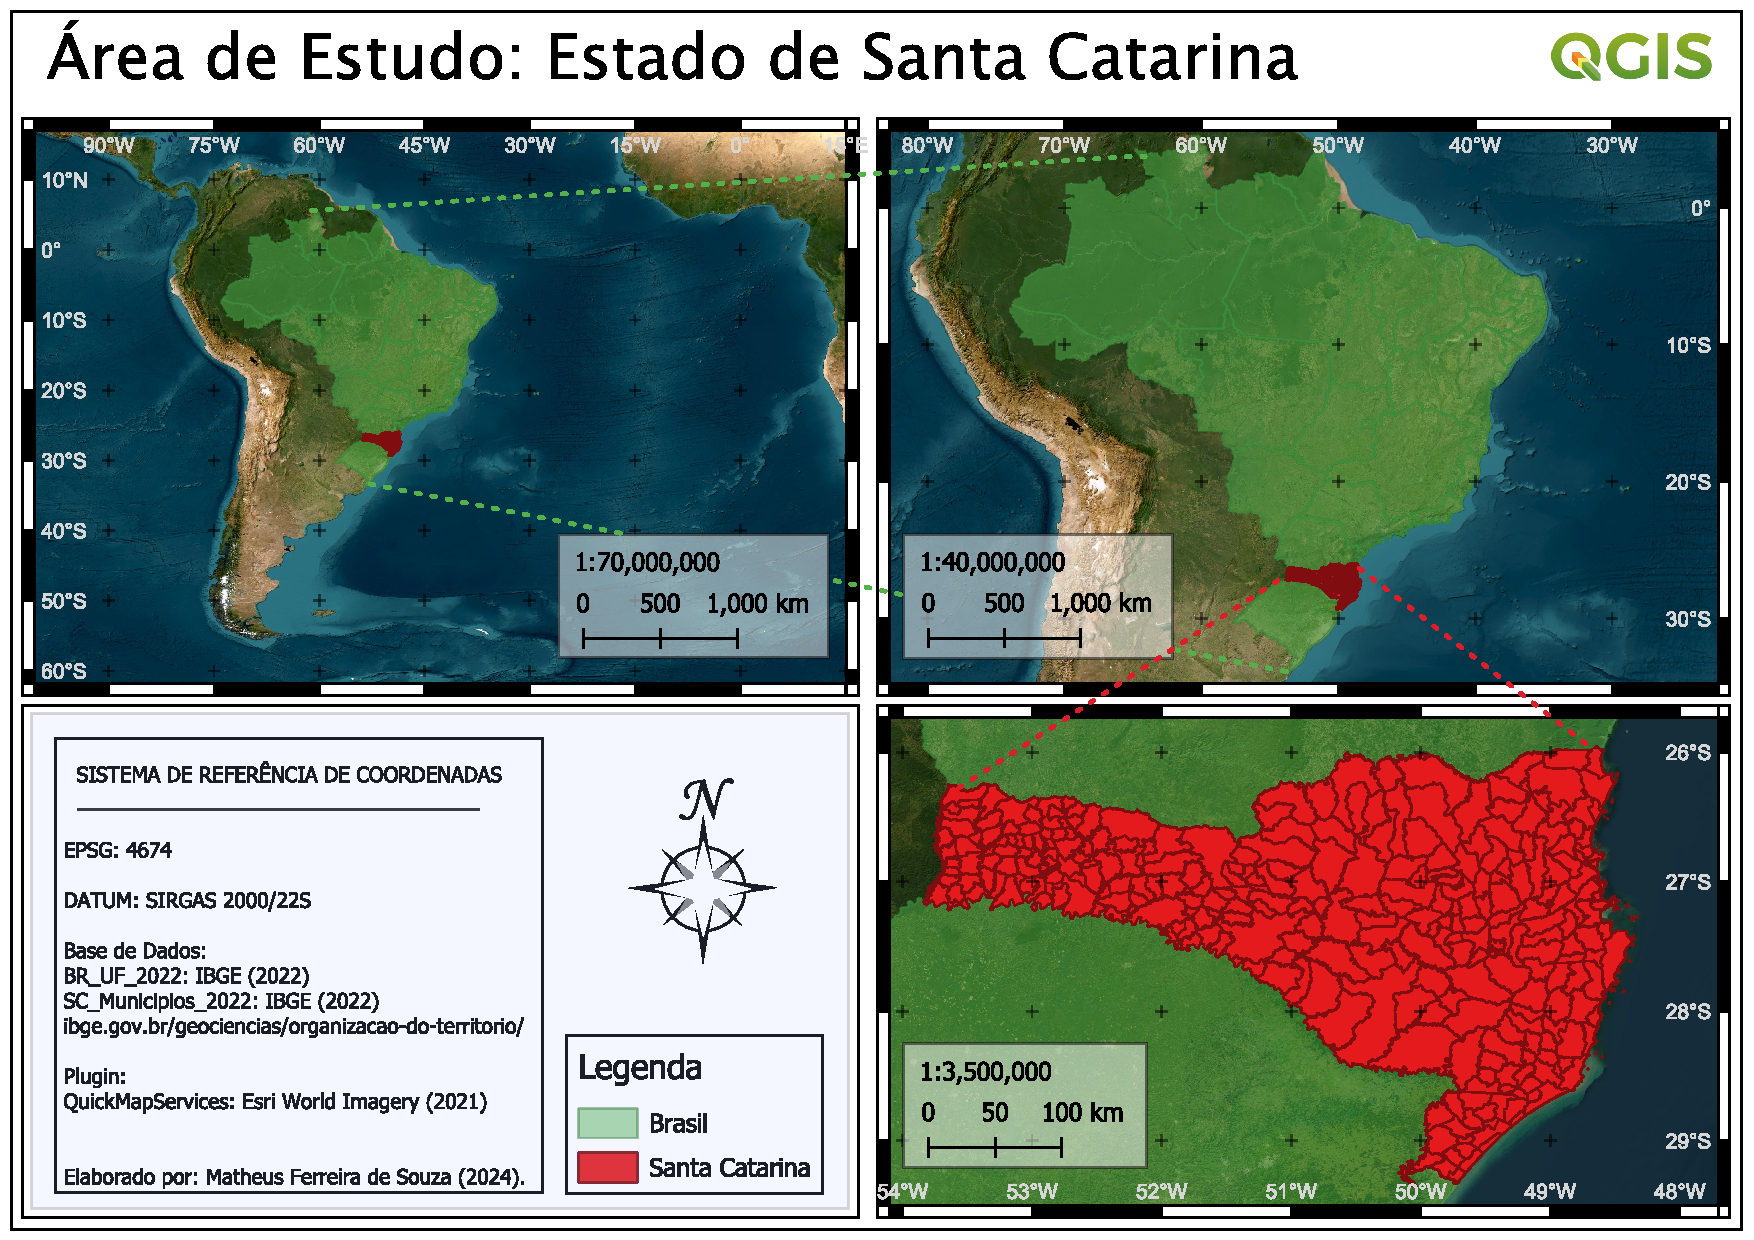
\includegraphics[scale=0.5]{figuras/area_de_estudo_SC_MATHEUS.pdf}
    \label{fig:area_de_estudo}
    \\
    \vspace{-0.05cm}\hspace{-7.5cm}\small{Fonte: Elaborado pelo próprio autor (2024).} 
\end{figure}

\indent Assim, o presente estudo realiza as análises descritiva e dignóstica dos elementos climáticos e entomo-epidemiológicos,  análise preditiva dos focos de \latim{Aedes} sp. e casos de dengue e, através deste projeto, cabe aos tomadores de decisão a realização da análise prescritiva.

\indent Para melhor explicação dos métodos, pretende-se dividir o estudo em etapas, relativas ao percurso de execução do próprio projeto, sendo: pré-processamento dos dados; análise estatística descritiva; modelagem preditiva e validação do modelo; espacialização dos dados preditos e estudo de casos; além de síntese do \acrfull{PTT}.


\section{Pré-processamento dos Dados}

Em relação aos \acrshort{DEE}, devem ser orientados ao modo que possam ser concatenados, adicionados, uma planilha após a outra. Para tal, utilizou-se a linguagem \ingles{Python} (versão 3) \cite{python3_2009_van}  e a biblioteca \ingles{pandas} \cite{pandas_2010_scipy, pandas_2020_reback}, como pacote principal para estruturação dos dados . Outras também foram utilizadas, como: \ingles{numpy} \cite{numpy_2020_harrisarray}, para tratar dados faltantes e tipagem de variáveis; \ingles{datetime} \cite{python2_1995_van}, para padronização de todas as datas e variáveis desse tipo; e \ingles{geopandas} \cite{geopandas_2020_kelseyjordahl}, para manipular arquivos georreferenciados, extrair deles a nomenclatura padrão dos municípios do \acrshort{IBGE} e aplicar aos próprios dados.\\
\indent Os \acrshort{DEC} foram previamente tratados utilizando o \ingles{\acrfull{CDO}} \cite{CDO_2023_schulzweida}, assim, pôde-se unir dados diários para composição de meses e anos, por fim, sintetizando a série histórica. Com esse mesmo \ingles{software} se fez o primeiro recorte espacial, para o sul do Brasil, diminuindo o tamanho do arquivo principal. Para abertura e manipulação dos arquivos climáticos, na extensão \ingles{netCDF4}, utilizou-se a biblioteca \ingles{xarray} \cite{xarray_2016_v0_8_0, xarray_2017_hoyer}.\\
\indent Após isso, foram extraídos os valores dos elementos climáticos de cada município e armazenados em um novo formato de arquivo, \ingles{\acrfull{csv}} (valores separados por vírgulas), utilizando as bibliotecas \ingles{pandas}, \ingles{numpy}, \ingles{geopandas} e \ingles{shapely} \cite{shapely_2007_gillies}.\\
\indent Finalmente,  os principais conjuntos de dados (temperatura mínima, temperatura média, temperatura máxima, precipitação, focos de \latim{Aedes} sp. e casos de dengue) eram próprios arquivos estruturados em tabela dinâmica, onde as colunas eram cada município catarinense e as linhas, a serié histórica dada em semanas epidemiológicas no formato \ingles{datetime64[ns](YYYY-mm-dd)}. Logo, a equiparação entre essas variáveis era possível.


\section{Análise Estatística Descritiva}

\indent \textcolor{red}{ARGUMENTAR COM O ADRIANO}

\indent \textcolor{red}{explicar como ocorreu a correlação.}

\indent Com os conjuntos de dados previamente estruturados, quatro (4) cidades foram elencadas para realizar análises de correlações. Alguns dados foram retroagidos em semanas epidemiológicas para melhor evidenciar possíveis correlações. Essas análises foram realizadas entre os \acrshort{DEE} (focos de \latim{Aedes} sp. e casos de dengue), entre esses elementos citados anteriormente e os \acrshort{DEC} (precipitação e temperaturas mínima, média e máxima), e entre os \acrshort{DEE} e limiares dos \acrshort{DEC}. A correlação propriamente dita foi calculada por meio do método \ingles{.corr()} da biblioteca \ingles{pandas}. Para melhor visualização do resultado desse cálculo, foram utilizadas as bibliotecas \ingles{numpy}, \ingles{matplotlib} \cite{matplotlib_2007_hunter} e \ingles{seaborn} \cite{seaborn_2021_waskom}.

\section{Modelagem Preditiva}

\indent Inicialmente, foram utilizados os pacotes \ingles{pandas}, \ingles{numpy} e \ingles{sklearn} \cite{scikit-learn_2011_pedregosa, sklearn_2013_buitinck}. Dessa maneira, os conjuntos de dados entomo-epidemiológicos e climatológicos foram estruturados em um único arranjo de dados para cada município. Essa estrutura foi composta pela variável dependente (entomológica ou epidemiológica) e por variáveis explicativas (elementos climáticos). Esse arranjo só foi possível com municípios que apresentavam todos os conjuntos de dados presentes. Sendo a variável dependente epidemiológica, é incluída a variável entomológica como explicativa. A configuração final do arranjo assumia, entre a variável dependente e as explicativas, horizonte preditivo de quatro (4) semanas epidemiológicas e retroação de oito (8) semanas epidemiológicas. Sendo a variável dependente epidemiológica, o horizonte preditivo de duas (2) semanas epidemiológicas e retroação de três (3) semanas epidemiológicas. Dessa última configuração, as variáveis explicativas (x) e dependente (y) foram divididas em dois conjuntos: treino e teste. Também foi previamente fixado um valor de gerador de números aleatórios (\ingles{seed}).

\indent \textcolor{red}{explicar como evitar "double dipping".}

\indent Após isso, com a utilização dos pacotes \ingles{tensorflow}\cite{tensorflow_2015_whitepaper} e \ingles{keras} \cite{keras_2015_chollet}, do próprio \ingles{tensorflow}, fez-se a instanciação do modelo de rede neural. A primeira camada incluída (camada zero (0)) faz o achatamento dos dados de entrada (variáveis explicativas). Logo, foram adicionadas duas camadas densas (camadas: um (1) e dois (2)) com dez (10) nós (neurônios) cada e ativadas por uma função \ingles{\acrshort{ReLU}} (unidade linear retificada). Então, acionou-se uma camada de regularização (camada três (3)) e uma camada densa de saída (camada 4 (4)). Essa última camada foi criada com a quantidade de nós suficientes para receber o valor de saída (variável dependente) e ativada por uma função \ingles{softmax}. Finalmente, o modelo foi compilado com otimização da taxa de aprendizagem (0,01), configuração de perda (entropia cruzada categórica esparsa) e de métrica (acurácia). Foi ajustado com 100 ciclos (épocas) máximos de treinamento e alocados 20 porcento (0,2) para validação, sendo que o número de ciclos durante a fase de treino foi limitado por um monitor de valor de perda, assim o treinamento encerra antes de 100 ciclos.

\indent Para o modelo \ingles{random forest}, utilizou-se o pacote \ingles{sklearn} e o mesmo conjunto de treino e teste das variáveis explicativas (x) e dependente (y). Ao compilar, foi atribuído um número total de árvores presentes (100) e o gerador de números aleatórios (previamente citado) para, então, ajustar aos conjuntos de treino das variáveis explicativas (x) e dependente (y).


\section{Validação/Verificação dos Modelos}

\indent \textcolor{red}{Histograma do Erro (Obs - Pre)\\
\indent Intervalo de Confiança para o Erro\\
\indent Raiz Quadrada do Erro Quadrático Médio (RQEQM)\\
\indent Erro Médio Absoluto (EMA)\\
\indent Viés = EMA - RQEQM\\
\indent Tempo de Execução Computacional}

\indent \textcolor{red}{ARGUMENTAR COM O ADRIANO}

\section{Espacialização dos Dados Preditos}

\indent Obteve-se os \ingles{shapefiles} do \acrshort{IBGE} (2022) para os limites territoriais (federal, estadual e municipais) do Estado de \acrlong{SC}. Para esse estudo, foi utilizado o recorte espacial durante a execução do prório \ingles{script}, sendo: longitude entre 54º5' e 57º5', ambas sul; e latitude entre 29º5' e 25º5', ambas oeste. Com esse recorte, pode-se evidenciar a totalidade do Estado de \acrlong{SC} e um pouco além de seus limites.

\indent Os modelos, previamente sintetizados, foram abertos através da biblioteca \ingles{joblib}, dos próprios desenvolvedores da biblioteca \ingles{sklearn}. Os dados de entrada são as próprias variáveis explicativas (x). Esses são abertos e estruturados pela biblioteca \ingles{pandas} e logo computados pela modelagem, retornando os valores de previsão da variável dependente (y).

\indent O centróide de cada município, que tenha algum valor de previsão, é incluído nesse novo conjunto de dados de retorno (previsão). O próprio centróide é padronizado ao Sistema de Referência de Coordenadas (\acrfull{CRS}) utilizado pelos \ingles{shapefiles} do \acrshort{IBGE} e o conjunto  de dados é transformado em \ingles{geodataframe} pela biblioteca \ingles{geopandas}. As semanas epidemiológicas também são transformadas em variável do tipo \ingles{datetime64[ns](YYYY-mm-dd)}.

\indent Para cada semana epidemiológica prevista, e através das bibliotecas \ingles{geopandas} e \ingles{matplotlib}, os valores calculados da variável dependente (y) foram atribuídos ao posicionamento geográfico de cada centróide, conforme \acrshort{CRS}, e sintetizado o mapa temático.

\textcolor{red}{Comentar sobre as diferenças na metodologia de mapa de calor e mapa coroplético?}
 
\section{Estudo de Caso}

\indent Quatro (4) cidades, escolhidas previamente à modelagem, foram utilizadas como estudo de caso para melhor entendimento dos próprios modelos.

\section{Síntese do \acrfull{PTT}} 

\indent Como preditivo da dinâmica entomológica de focos de \latim{Aedes} sp. e epidemiológica de casos de dengue no Estado de \acrlong{SC}, o \acrshort{PTT} resultante será:

\begin{itemize}
  \item o sistema computacional;
  \item visualização cartográfica desses resultados.
\end{itemize}

\indent O limiar temporal estipulado para previsão de focos de \latim{Aedes} sp. será de 56 dias (8 semanas epidemiológicas). Os primeiros 28 dias (4 semanas epidemiológicas) serão determinados a partir do sistema \acrshort{SAMeT}-\acrshort{MERGE}. Os demais dias/semanas epidemilógicas serão determinados através do \textcolor{red}{modelo de previsão \acrshort{GFS}.}

\indent O limiar temporal estipulado para previsão de casos de dengue será de 28 dias (4 semanas epidemiológicas). Os primeiros 14 dias (2 semanas epidemiológicas) serão determinados a partir do sistema \acrshort{SAMeT}-\acrshort{MERGE}. Os demais dias/semanas epidemiológicas serão determinados através do \textcolor{red}{modelo de previsão \acrshort{GFS}.}


%\section{Conjutos de Dados Utilizados}
%sobre as arboviroses emergentes e re-mergentes (\textbf{Dengue}, Febre Amarela, Zika, Chikungunya)
%Tornar cada parte do método em objetivo específico
%ATUALIZAR, PENSANDO NO PROCESSO FUTURO\\


%A princípio, os dados de regionalização espacial encontram-se em processo de definição.




% \subsection{Pré-processamento dos Dados}
% \indent Para desenvolvimento do trabalho, os dados foram ajustados em mesma escala temporal, deixando-os em semanas epidemiológicas. Dessa forma, fez-se o somatório dos registros de focos de \latim{Aedes} sp. por semana epidemiológica. Mesmo tratamento foi realizado com a precipitação, retornando o acumulado de precipitação por semana epidemiológica. As temperaturas foram agrupadas de forma diferente, porém também ajustando a dados semanais. Ao final, teríamos a média das temperaturas (mínima, média e máxima) por semana epidemiológica.\\


